\input{../std.tex}

\begin{document}
  \begin{center}
    \LARGE \textbf{Física Computacional} \\
    \Large \textbf{Tarefa 7 - Questão 6} \\
    \large Alex Enrique Crispim
  \end{center}

  Para $F_d = 1.2$ e duas condições iniciais diferente para $\theta$ (0.2 e 0.2-0.003), o gráfico de $\abs{\Delta \theta} \times t$, com o eixo vertical é mostrado na imagem abaixo.

  \begin{figure}[h]
    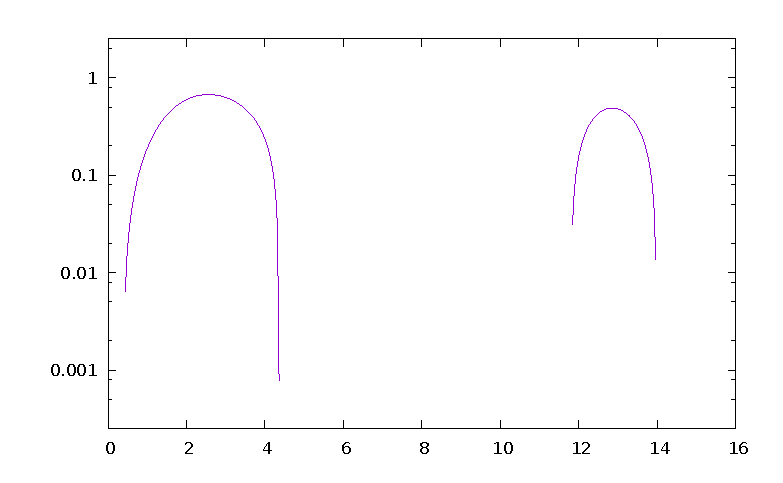
\includegraphics{LogDif}
  \end{figure}

  Podemos aplicar o método RK4 e apenas calcular $\abs{\Delta \theta}$. Da figura, podemos ver que nos picos de oscilação, as duas funções diferem tal que o logaritmo se apoxima de 1. Isso representa quando o logaritmo se torna igual a variação entre as duas funções. 


\end{document}
